\documentclass[11pt,a4paper,twoside,final]{report}
%

\usepackage{ngerman}            %Neue Rechtschreibung
\usepackage{graphicx}           %Graphiken einbinden
\usepackage[normalsize]{subfigure}
\usepackage[T1]{fontenc}            %Verwenden von \"{o} \"{a} \"{u} {\ss}
\usepackage[latin1]{inputenc}   	%Verwenden von �, �, �, �
\usepackage{fancyhdr}           %Kopf-und Fusszeilen
\usepackage{theorem}
\usepackage{amsmath}
\usepackage{amssymb}
\usepackage{bibgerm}
\usepackage{parskip}
\usepackage{longtable}
\usepackage{helvet}
\usepackage[right]{eurosym}
\usepackage{pdflscape}
\usepackage[compact]{titlesec}
\usepackage{tikz}
\usepackage{lmodern}

\usetikzlibrary{positioning}
\usetikzlibrary{calc}
\usetikzlibrary{shapes.geometric}
\usetikzlibrary{shapes.arrows}
\usetikzlibrary{decorations}
\usetikzlibrary{decorations.pathmorphing}
\usetikzlibrary{decorations.text}
\usetikzlibrary{decorations.markings}
\usetikzlibrary{backgrounds}
\usetikzlibrary{intersections}

\usepackage[a4paper,
			textwidth = 16.5cm,
			textheight = 25cm,
			inner = 2.5cm]{geometry}
		
		
\usepackage[pdftex,
			colorlinks,
			linkcolor = black,
			citecolor = black]{hyperref}
%
%--------------------------------------------------------------------
%
%Kopf- und Fu�zeile
%
\pagestyle{fancyplain}
 \renewcommand{\chaptermark}[1]{\markboth{#1}{}}
 \renewcommand{\sectionmark}[1]{\markright{\thesection\ #1}}
 \lhead[\fancyplain{}{\sl\thepage}]{\fancyplain{}{\sl\rightmark}}
 \rhead[\fancyplain{}{\sl\leftmark}]{\fancyplain{}{\sl\thepage}}
 \lfoot{}
 \cfoot{}
 \rfoot{}
%--------------------------------------------------------------------
%
%Definition der Abschnitts�berschriften
%
%\titleformat{\chapter}[hang]{\normalfont{}\bfseries}{\thechapter}{10pt}{\large}{}
%\renewcommand{\thesection}{\alph{section}}
%\titleformat{\section}[runin]{\normalfont}{\thesection )}{6pt}{}
%
%--------------------------------------------------------------------
%
%Kommandos f�r die Titelseitendaten
%
\newcommand{\VersuchNummer}[1]{\newcommand{\VNummer}{#1}}
\newcommand{\VersuchName}[1]{\newcommand{\VName}{#1}}
\newcommand{\Name}[1]{\newcommand{\SName}{#1}}
\newcommand{\Studiensemester}[1]{\newcommand{\SSemester}{#1}}
\newcommand{\VersuchDatum}[1]{\newcommand{\VDatum}{#1}}
\newcommand{\Mitarbeiter}[1]{\newcommand{\VMitarbeiter}{#1}}
%
%--------------------------------------------------------------------
%
%Titelseite
%
%Daten zum Versuchsprotokoll f�r das Praktikum Elektrische Antriebe
%
%Eingegeben werden:
%
% - Die Nummer und Name des Versuchs:
%     1 Asynchronmaschine
%     2 Gleichstrommaschine
%     3 B�rstenloser Gleichstrommotor
%     4 Schrittmotor
%
\VersuchNummer{1}
\VersuchName{Beschreibung der Komponenten}
%
%------
%
% - Name des Bearbeiters
%
\Name{}
%
%------
%
% - Studiensemester des Bearbeiters
\Studiensemester{6}
%
%------
%
% - Datum der Versuchsdurchf�hrung
%
\VersuchDatum{22.05.2016}
%
%------
%
% - Namen der Mitarbeiter in der Gruppe
%
\Mitarbeiter{Benjamin Haid, Marius Ketterer, Tobias Soldan, Steffen Wandel}
%
\renewcommand\maketitle{
\begin{titlepage}

\thispagestyle{empty}
%
\begin{tabular}[t]{lp{0.25\textwidth}r}
%

\includegraphics[width = 0.25\textwidth]{./Bilder/Logo_HSRT_TEC_RGB.png}
%
&&
\includegraphics[width = 0.4\textwidth]{./Bilder/Logo_HSRT_Schwarz.jpg}
%
\end{tabular}
%

\renewcommand{\baselinestretch}{1.2}

\sf\large\textbf{Hochschule Reutlingen}\\
\sf\large\textbf{Fakult�t Technik}\\

\vspace{7cm}

{\sf\Huge\textbf{Regelungstechnik Projekt}}\\
%
\vspace{0.5cm}

{\sf\huge{Bericht~\VNummer:}}\\
{\sf\huge{\VName}}

\vspace{4.5cm}

\renewcommand{\arraystretch}{2}
\begin{tabular}{|p{0.33\textwidth}p{0.33\textwidth}p{0.33\textwidth}|}
%
\hline
\multicolumn{2}{|p{0.66\textwidth}|}{Name:~\SName}				&Studiensemester:~\SSemester		\\
\hline
Datum:~\VDatum			      &\multicolumn{2}{|l|}{Testat:}		\\
\hline
\multicolumn{3}{|l|}{Mitarbeiter:~\VMitarbeiter}\\
\hline
%
\end{tabular}
\renewcommand{\arraystretch}{1}

\renewcommand{\baselinestretch}{1}
%

\vfill
%


\includegraphics[width = \textwidth]{./Bilder/Silhouette_HSRT_045K.jpg}
%
\newpage
\ 
\thispagestyle{empty}
%
\end{titlepage}}
%
%--------------------------------------------------------------------
%
\begin{document}
%
\maketitle
\setcounter{page}{1}

%--------------------------------------------------------------------
%
%Mustervorlage fuer eine Aufgabe
%
%--------------------------------------------------------------------
%
%Ueberschreiben der automatisch erzeugten Aufgabennummer
%Die folgende Aufgabennummer ergibt sich aus dem Stand des
%Z�hlers + 1
%\setcounter{chapter}{0}
%
\chapter{Blockschaltbild}\label{ex:blockschaltbild}
%
%Teilaufgabe 1
%
\section{}\label{sec:blockschaltbild}
%
Hier sehen Sie das Blockschaltbild des gesamten Systems (Abb. \ref{pic:blockschaltbild}):

\begin{figure}[htb]
%
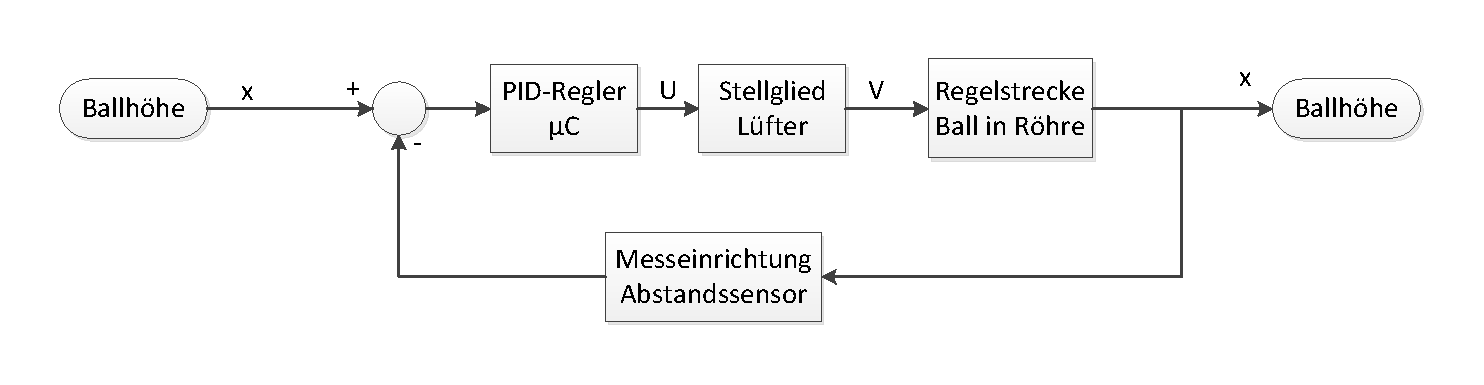
\includegraphics[width = \textwidth]{./Bilder/Blockschaltbild}
\caption{Blockschaltbild des Systems}
\label{pic:blockschaltbild}%
\end{figure}

%
%--------------------------------------------------------------------
%
%Teilaufgabe 2
%
\section{}\label{sec:einsinnvolleslabel1}
%

%
%Alle bisherigen Bilder einf�gen und einen Seitenumbruch erzwingen
\clearpage

@@ -0,0 +1,52 @@
%--------------------------------------------------------------------
%
%Mustervorlage fuer eine Aufgabe
%
%--------------------------------------------------------------------
%
%Ueberschreiben der automatisch erzeugten Aufgabennummer
%Die folgende Aufgabennummer ergibt sich aus dem Stand des
%Z?hlers + 1
%\setcounter{chapter}{0}
%
\chapter{Beschreibung der �bertragungsfunktionen}\label{ex:uebertrag}
%
%Teilaufgabe 1
%
\section{Regelstrecke}\label{sec:regelstrecke}
%
Ausgehend von dem Gleichgewicht der Kr�fte $F_Z + F_R - m*g - m*a = 0$\\
Daraus ergibt sich folgende Differentialgleichung:
\begin{equation}
	\frac{32\mu_0 l^*}{\rho v D^{*^2}} \rho v^2 A + 6\pi \mu_0 vr - mg = m \ddot{x}
\end{equation}
Nach K�rzen ergibt sich:
\begin{equation}
\frac{32\mu_0}{D^*} v A + 6\pi\mu_0 vr - mg = m\ddot{x}
\end{equation}
Nach der Laplacetransformation erh�lt man:
\begin{equation}
\frac{32\mu_0}{D^*} v A + 6\pi\mu_0 vr - mg = m *\text{s}^2 x
\end{equation}
Umgestellt nach dem Weg:
\begin{equation}
\frac{1}{\text{s}^2} * (\frac{32\mu_0}{m D^*} v A + \frac{6\pi\mu_0 vr}{m} - g) = x
\end{equation}
%
Das Ergebnis wird mittels Einheiten gepr�ft:
\begin{equation}
\frac{\mu_0 v A}{mD^*} = \frac{[Pa*s * m * m^2]}{[kg * m]} = \frac{[N * m^4 * s]}{[N * s^3 * m^3]} = \frac{[m]}{[s^2]}
\end{equation}
\begin{equation}
	\frac{\mu_0 v r}{m} = \frac{[Pa*s*m*M]}{[kg*s]} = \frac{[N*m^3*s]}{[N*s^3*m^2]} = \frac{[m]}{[s^2]}
\end{equation}
\begin{equation}
	g = \frac{[m]}{[s^2]}
\end{equation}
Die Beschleunigung zweimal integriert ergibt den Weg.
%--------------------------------------------------------------------
%
%
\newpage
\section{Abstandssensor}
%
Durch Linearisierung im Arbeitspunkt x = 45 cm ergibt sich folgende �bertragungsfunktion:
\begin{equation}
	U(x) = -1.25x + 1.25
\end{equation}
\section{L�fter}
Durch Linearisierung im Arbeitspunkt \textit{U} = 5V ergibt folgende �bertragungsfunktion:
\begin{equation}
U(x) = -0.018x + 0.13
\end{equation}
%Alle bisherigen Bilder einf?gen und einen Seitenumbruch erzwingen
\clearpage
\chapter{Aufbau}
\section{Elektrischer Aufbau}




\section{Mechanischer Aufbau}\label{sec:mechanischer_Aufbau}
	\subsection{St�ckliste}
	\begin{enumerate}
		\item Plexiglasrohr
		\item Plexiglasscheibe
		\item 4 M6 Schrauben
		\item 8 M6 Muttern
		\item 8 M6 Unterlagsscheiben
		\item Anschlussteil einen HT-Abwasserrohrs
		\item L�fter
		\item Abstandssensor
		\item Patex 2K Kleber
		\item Sekundenkleber
	\end{enumerate}
\subsection{Beschreibung}
Die Plexiglasscheibe dient als Basis des gesamten mechanischen Aufbaus (siehe Abb. \ref{fig:Aufbau_gesamt}). In ihrer Mitte befindet sich ein Loch durch welcher das HT-Rohr, bis zur Dichtungsverbreiterungs, genau durchpasst. Obwohl das HT-Rohr schon durch eine Presspassung in der Plexiglasscheibe h�lt wurde es zus�tzlich mit Zweikkomponentenkleber fixiert. In die vier Ecken der Scheibe wurde L�cher gebohrt, durch diese wurden die Schrauben gesteckt und mit den Mutter sowie den Unterlagsscheiben fixiert. Die Schrauben dienen Als F��e f�r den Aufbau. Dies hat fogende Vorteile:
\begin{itemize}
		\item Der L�fter liegt nicht dirkt auf dem Untergrund und kann somit Luft ansaugen.
		\item Der Aufbau steht stabil auf dem Untergrund.
		\item Durch die Verwendung von Schrauben kann ein unebener Untergrund ausgeglichen werden.
\end{itemize}

In die Verbreiterung des HT-Rohrs befindet sich normalerweise eine Gummidichtung. In unserem Fall kann dort aber der L�fter bequem eingeclipst werden. Auf dem L�fter wurde der Abstandssensor mit Sekundenkleber befestigt. Da der Sensor einen Steckanschluss hat und dieser im fertigen Aufbau nicht mehr erreicht werden kann, wurde dieser mit Litzen, am L�fter vorbei unten aus dem HT-Rohr gef�hrt. In das andere Ende des HT-Rohrs wird das Plexiglas Rohr gesteckt werden, dieses passt ebenfalls genau dort hinein und ist somit durch eine Presspassung fixiert (siehe Abb. \ref{fig:IMG_20160523_191318}).

\begin{figure}[!htb]
	\centering
	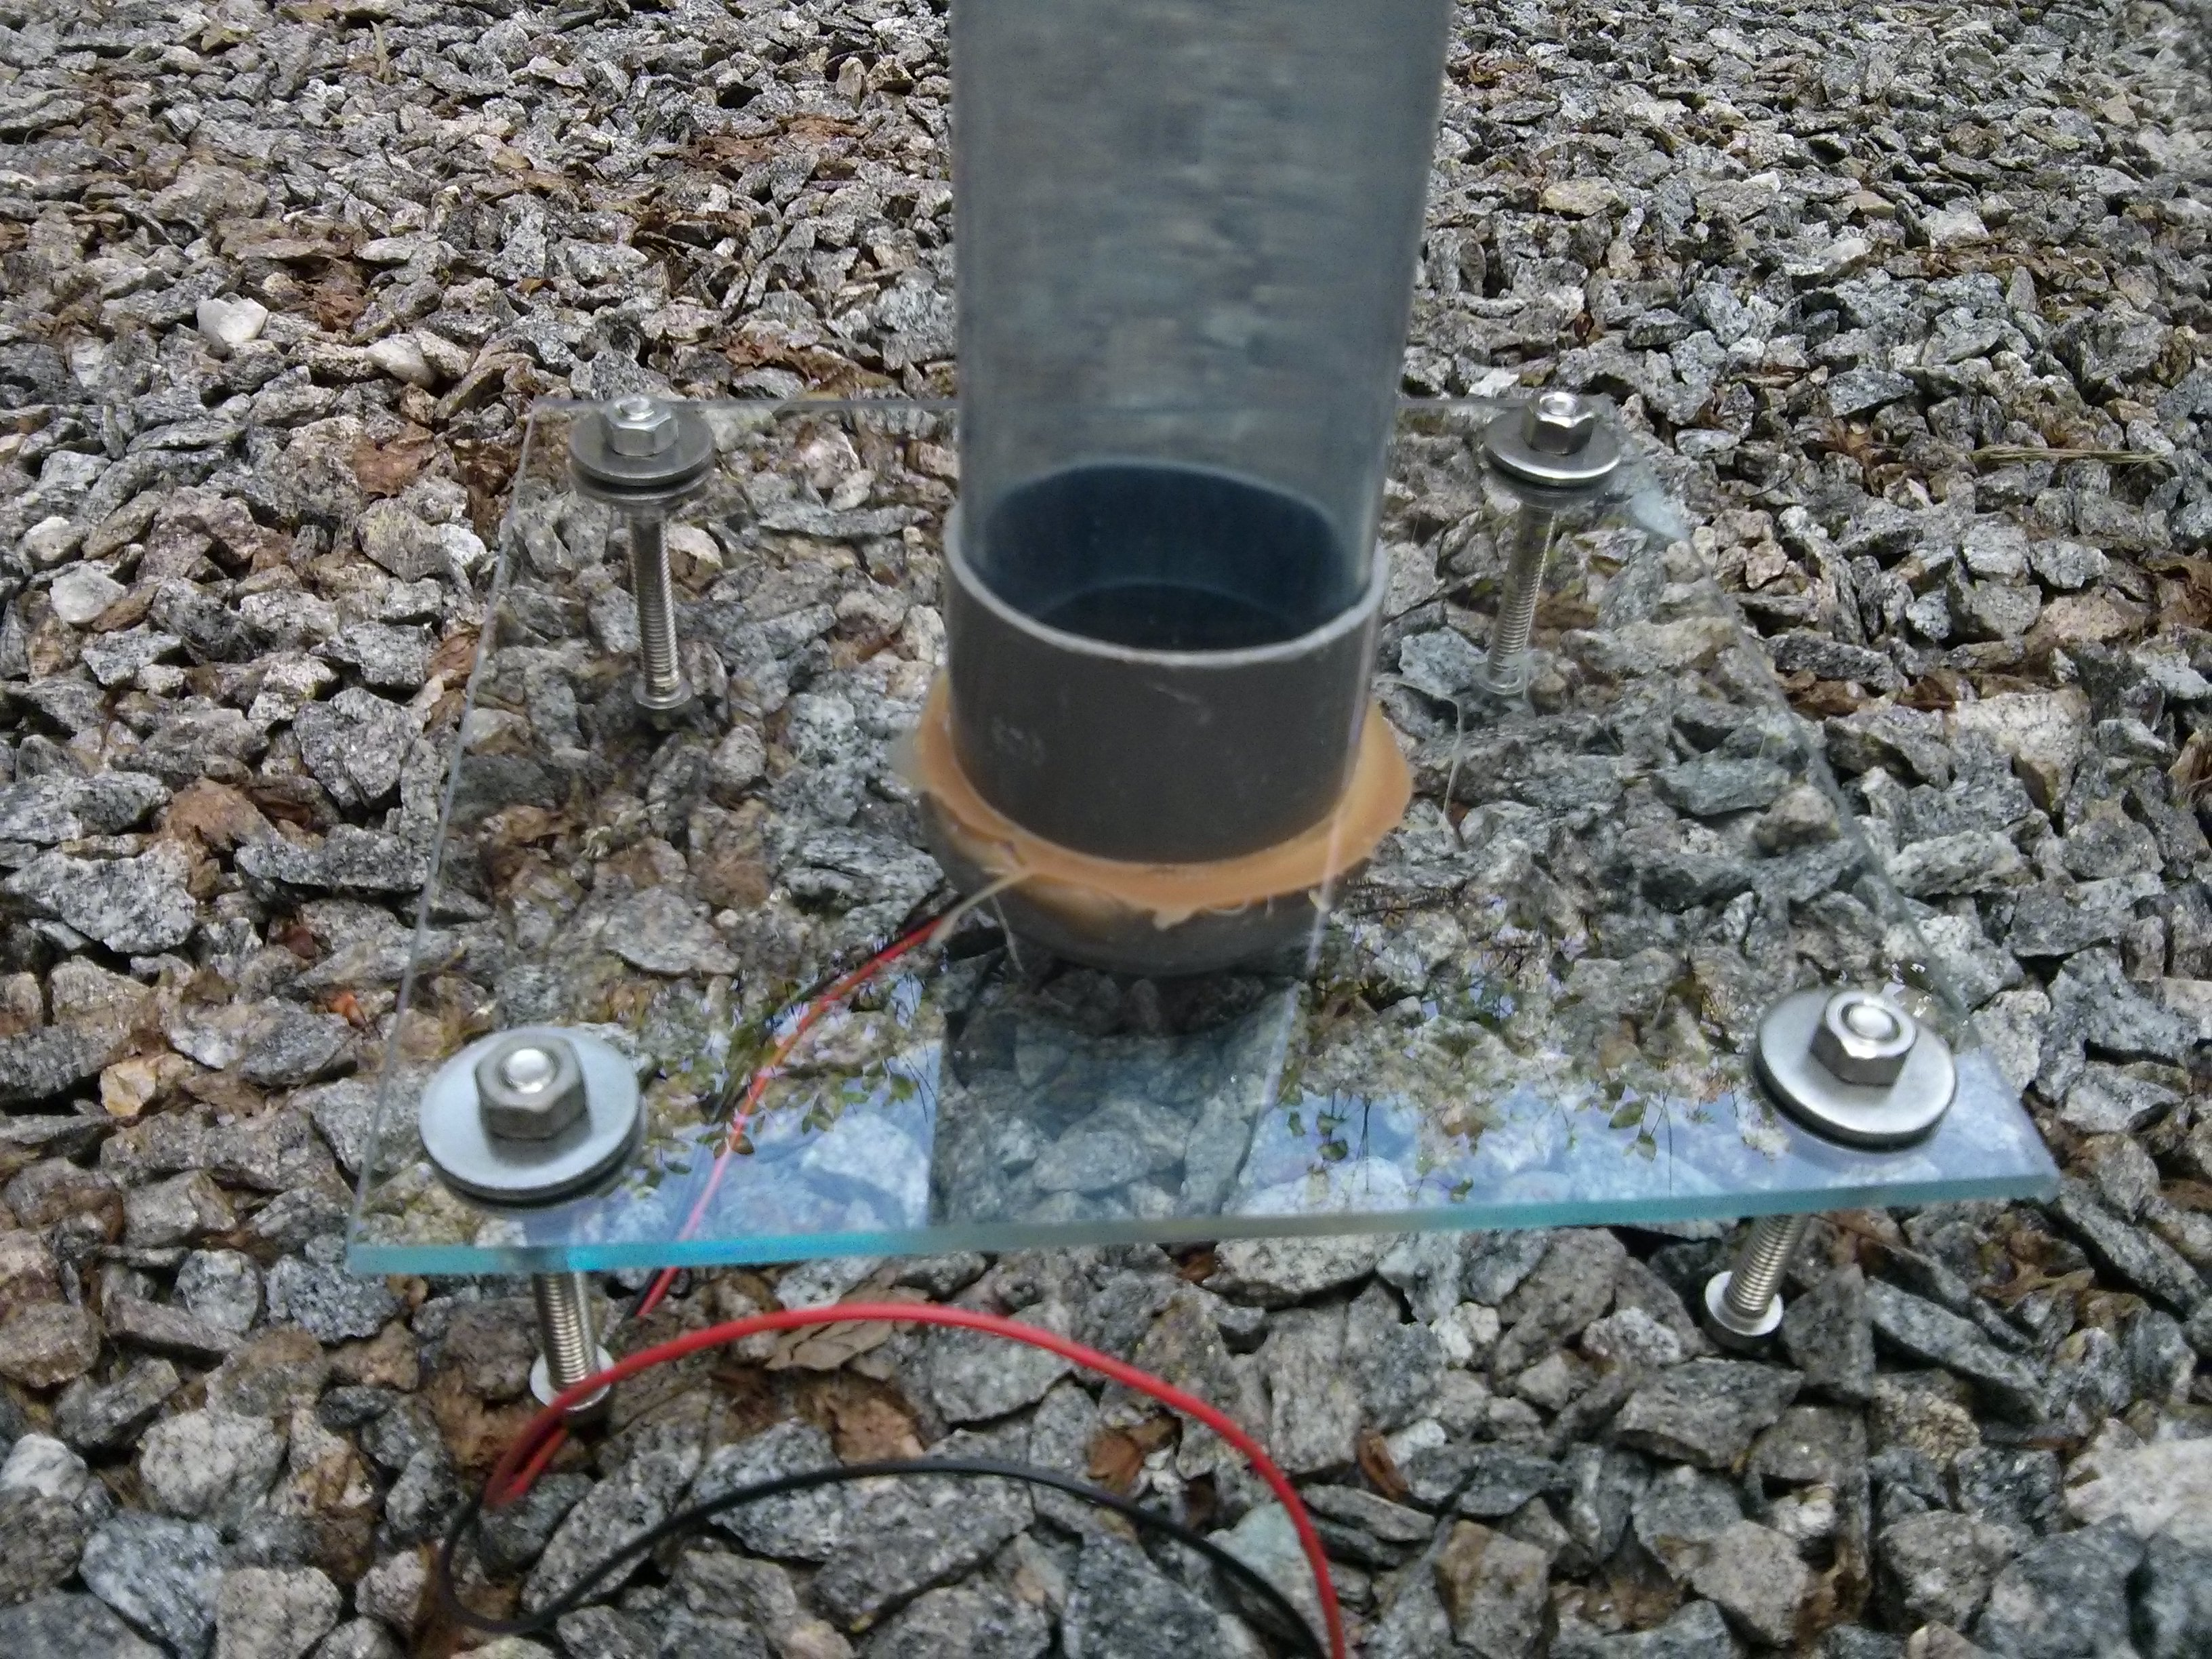
\includegraphics[width=0.8\linewidth]{./Bilder/IMG_20160517_152455}
	\label{fig:Aufbau_gesamt}
	\caption{Fertiger mechanischer Aufbau}
\end{figure}
\begin{figure}[!htb]
	\centering
	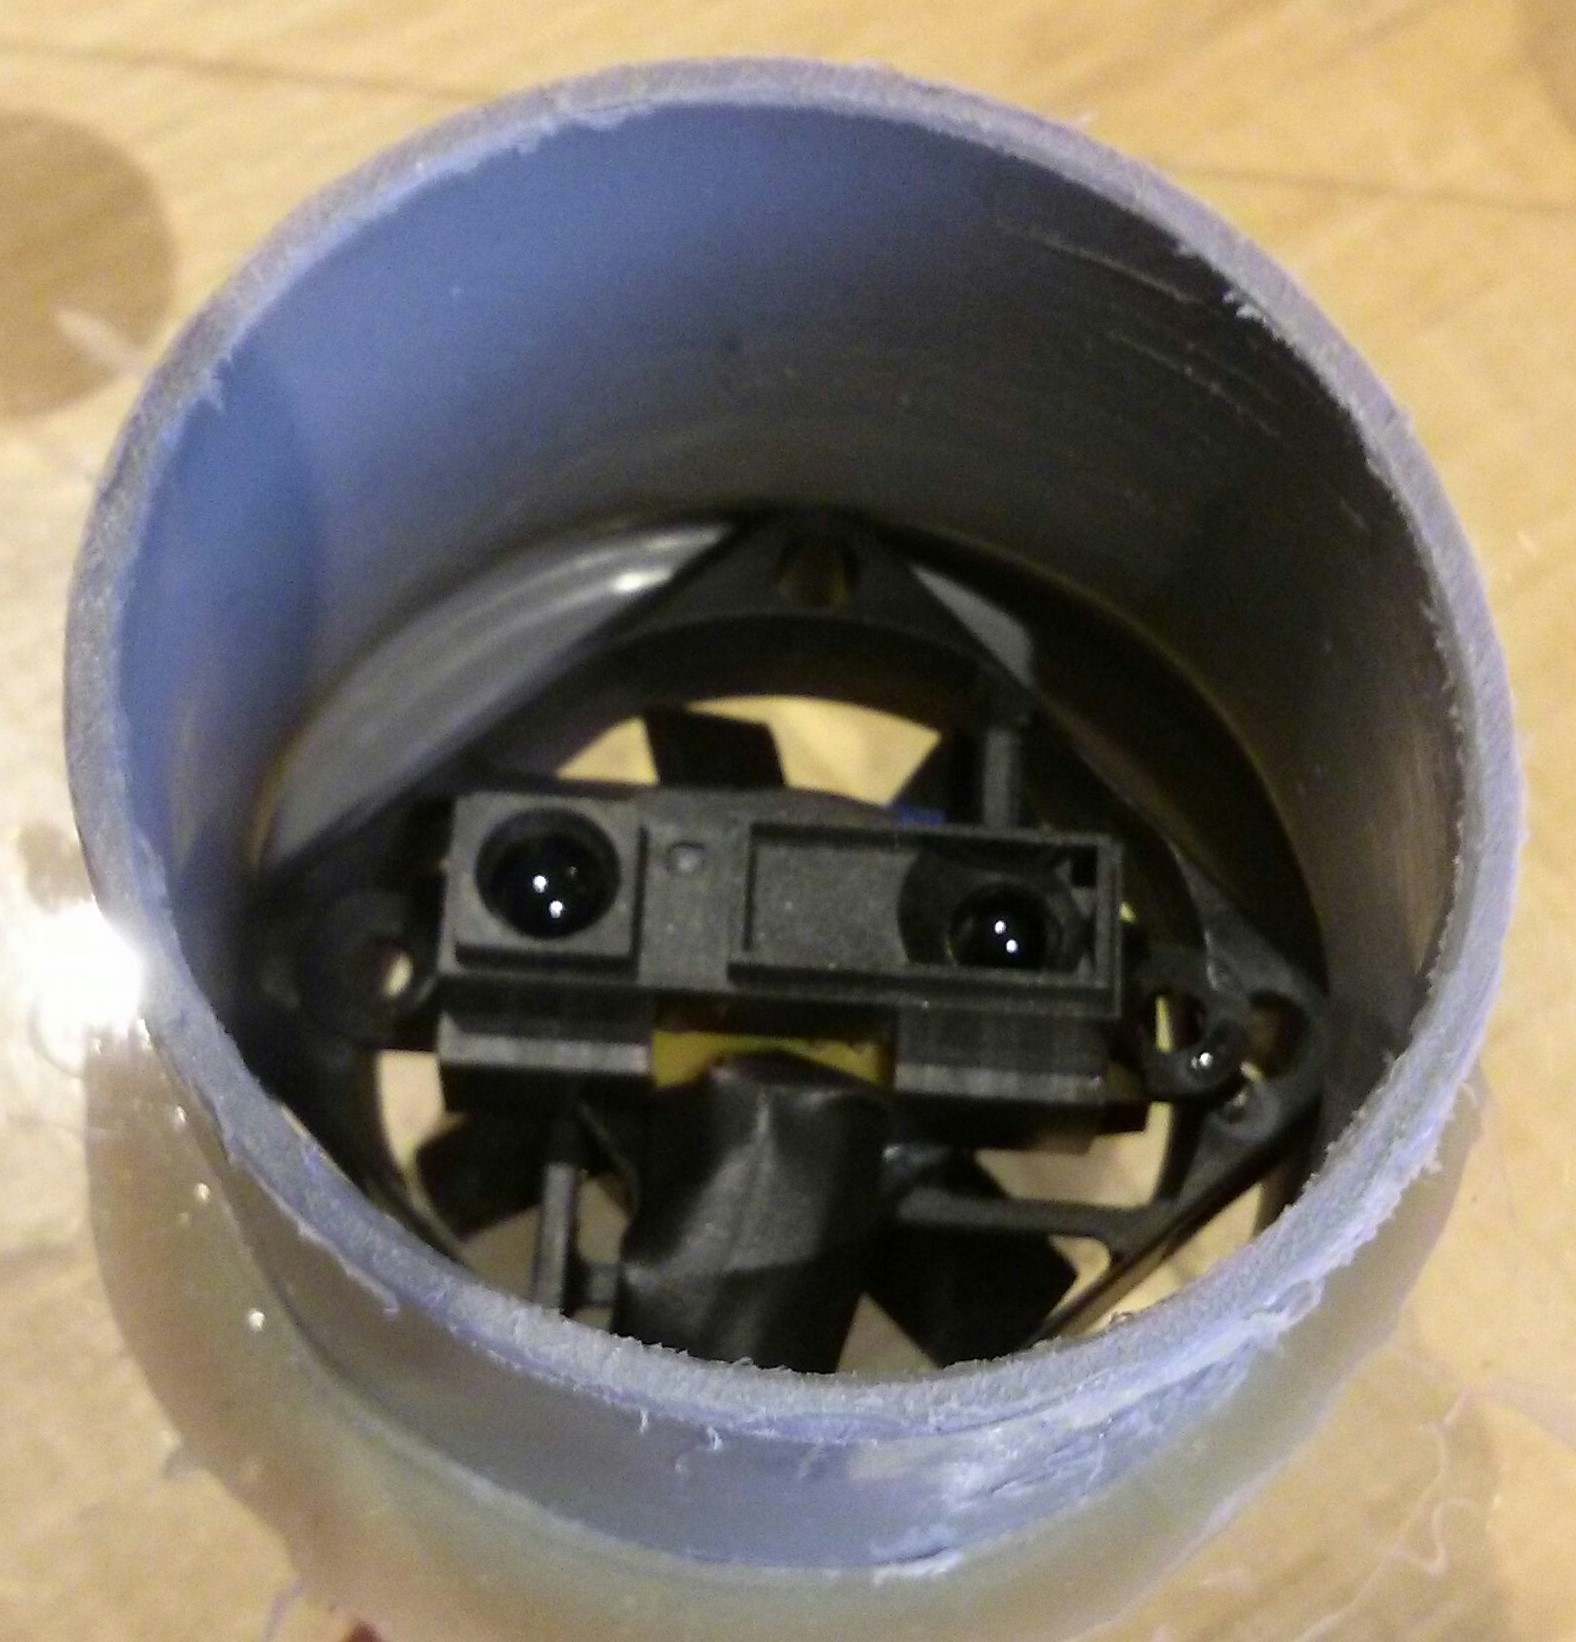
\includegraphics[width=0.6\linewidth]{./Bilder/Luefter_mit_Sensor_im_Rohr}
	\caption{L�fter mit Sensor im HT-Rohr}
	\label{fig:IMG_20160523_191318}
\end{figure}



\chapter{Verbesserungen und Anmerkungen}
\section{Mechanischer Aufbau}
Bei einem ersten Versuch mit dem mechanischen Aufbau wie er in \ref{sec:mechanischer_Aufbau} beschrieben wurde. Wurde festgestellt dass wenn der Sensor direkt auf dem Lüfter befestigt wird, reicht der erzeugte Luftstrom nicht aus um den Ball anzuheben. Daher folgende Verbesserungen in Betracht gezogen:
\begin{itemize}
	\item Sensor mit ca. 20mm Abstand zum Lüfter befestigen.
	\item Versuchen das Sensorgehäuse zu verkleinern, z.B. durch abscheiden überflüssiger Plastikteile.
\end{itemize}
%
%und m�glicherweise noch andere Aufgaben
%

%
\end{document}

